\section{Dust Empirical Modeling} \label{sec:methods}
\subsection{Fiducial DEM} \label{sec:dem}
\todo{motivation for the DEM model} 

\cite{trayford2015} uses an empirical dust model but doesn't implement an
attenuation curve but rather multiplicative factors for the broadband
photometry.

We begin by defining the dust attenuation curve $A(\lambda)$ as 
\begin{equation} 
    F_o (\lambda) = F_i (\lambda) 10^{-0.4 A(\lambda)}
\end{equation}
where $F_o$ is the observed flux and $F_i$ is the intrinsic flux. We normalize the attenuation at the $V$ band, 
\begin{equation} 
    A(\lambda) = A_V \frac{k(\lambda)}{k_V}. 
\end{equation}

For the normalization of the attenuation curve, $A_V$, we use the slab model
from~\cite{somerville1999, somerville2012}. In the slab model the amplitude of
attuenuation depends on the inclination angle, $i$, and the optical depth,
$\tau_V$: 
\begin{equation} \label{eq:slab}
    A_V = -2.5 \log \left[ \frac{1 - e^{-\tau_V\,\sec i}}{\tau_V\,\sec i} \right]
\end{equation}
\todo{justification of why this is enough}. We sample $i$ uniformly.
% is the slab model consistent with Battisti et al. (2017b) who find a
% correlation with the attenuation curve slopes: highly inclined galaxies have shallower slopes (S = 2.2) with a possible weak bump (B ∼ 0.1), whereas face on galaxies had steeper slopes (though still only S = 2.7)


% at fixed A_ISM, higher inclination (more edge-on) galaxies exhibit greyer V attenuation curves. Taking the difference in this way removes the primary trend that higher AISM measurements tend to be associated V with more edge-on galaxies. This effect has been previously noted for real galaxies (e.g. Wild et al. 2011), and attributed to the effect that the attenuation in face-on galaxies is governed by the physical association between ISM and young stars, while in edge- on systems dust lanes are less discriminating between differently aged populations.

%Salim+(2020): explanatiion for why we don't have slope depend on inclination. 
%Remarkably, the lack of difference in the slopes at fixed AV is true even for
%galaxies with very different inclinations. A dusty galaxy with a face-on
%attenuation of AV and a less dusty galaxy that has the same AV (because we
%observe it edge-on) will have the same attenuation curve slope, as predicted
%in the radiative transfer models analyzed by Chevallard et al. (2013).
% Salim+(2020): We conclude that the dominant determinant in the slope of the
% attenuation curve, out of the considered physical parameters, is AV .

Recently, \cite{salim2020} find significant dependence in $A_V$ on both $M_*$
and SFR. We include this dependence through $\tau_V$, which we flexibly
parameterize as 
\begin{equation} \label{eq:tauv}
    \tau_V(M_*, {\rm SFR}) = m_{\tau,1} \log \left(\frac{M_*}{10^{10} M_\odot}\right) +
    m_{\tau,2} \log\,{\rm SFR} + c_\tau.
\end{equation}

Next, for the wavelength dependence of the attenuation curve, we use $k(\lambda)$ from 
\cite{noll2009}: 
\begin{equation} \label{eq:noll}
    k(\lambda) = \left(k_{\rm Cal}(\lambda) + D(\lambda)\right) \left(
    \frac{\lambda}{\lambda_V} \right)^\delta.
\end{equation}
Here $k_{\rm Cal}(\lambda)$ is the \cite{calzetti2001} curve: 
\[
    k_{\rm Cal}(\lambda) = 
    \begin{cases} 
        2.659 (-1.857 + 1.040/\lambda) + R_V, & 6300 \AA \le \lambda \le
        22000 \AA \\ 
        2.659 (-2.156 + 1.509/\lambda - 0.198/\lambda^2 + 0.011/\lambda^3) +
        R_V & 1200 \AA \le \lambda \le 6300 \AA
    \end{cases}
\]
where $\lambda_V$ is the $V$ band wavelength. $\delta$, the slope of the attenuation curve.
also correlates with galaxy
properties.
So we parameterize $\delta$ and 
\begin{align}
    \delta(M_*, {\rm SFR}) &= m_{\delta,2} \log \left(\frac{M_*}{10^{10}
    M_\odot}\right) + m_{\delta,2} \log\,{\rm SFR} + c_\delta 
\end{align}

$D(\lambda)$ is the UV dust bump, which we
parameter using the standard Lorentzian-like Drude profile:
\begin{equation}
    D(\lambda) = \frac{E_b(\lambda \Delta \lambda)^2}{(\lambda^2 -
    \lambda_0^2)^2 + (\lambda \Delta \lambda)^2}
\end{equation}
where $\lambda_0$, $\Delta \lambda$, and $E_b$ are the central wavelength,
FWHM, and strength of the bump, respecitvely. In our DEM, we assume fixed 
$\lambda_0 = 2175 \AA$ and $\Delta \lambda = 350\AA$. 

\cite{kriek2013} and \cite{tress2018} found evidence that $E_b$ correlates with
the slope of the attenuation curve for star-forming galaxies $z\sim2$. This was
dependence was confirmed with simulations in \cite{naranyanan2018}. $E_b$: 
\begin{align} \label{eq:bump_amp}
    E_b &= m_E~\delta + c_E
\end{align}
\todo{we fixed this and find our results do not change significantly.} 

We also split the attenuation on the star light and nebular emission 
\begin{equation} 
    F_o (\lambda) = F^{\rm star}_i (\lambda) 10^{-0.4 A(\lambda)} + F^{\rm
    neb}_i (\lambda) 10^{-0.4 A_{\rm neb}(\lambda)}
\end{equation}
where we parameterize
\begin{equation}
    A_{\rm neb}(\lambda) = f_{\rm neb}  A(\lambda) 
\end{equation} 

\todo{mention of how we treat SFR = 0 galaxies} 

\begin{figure}
\begin{center}
    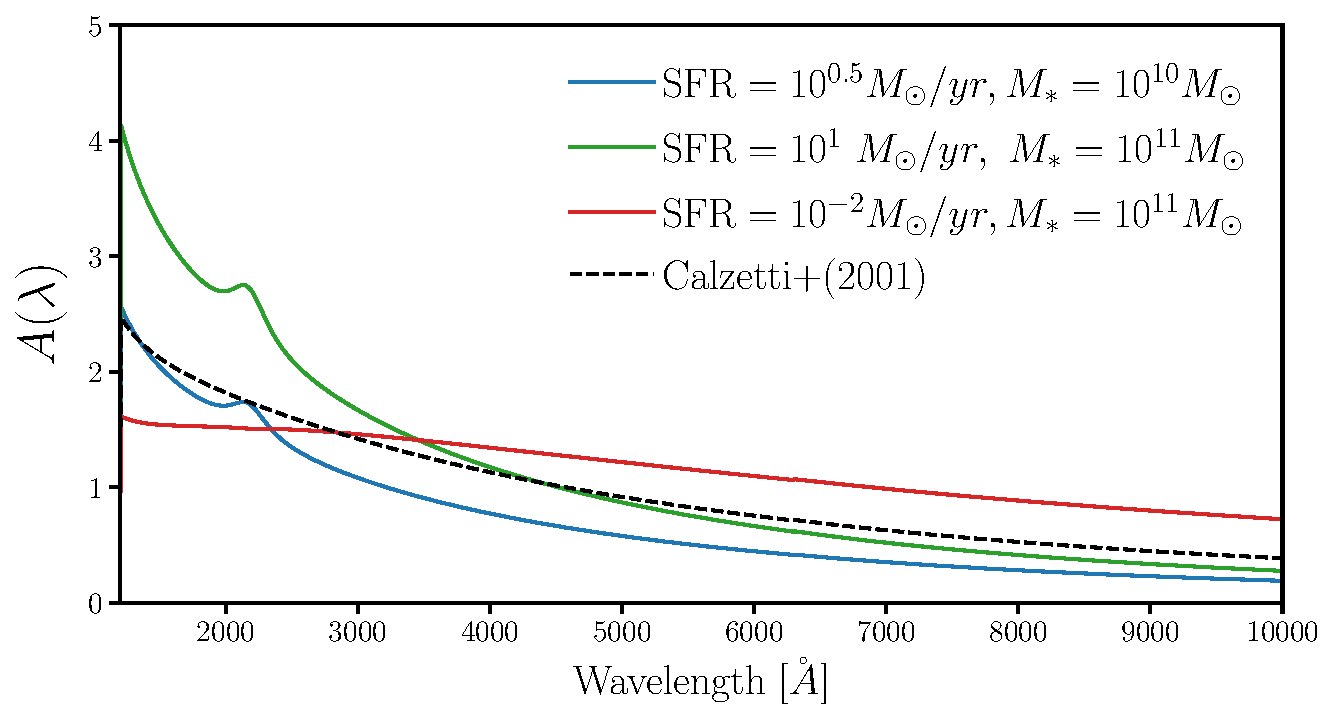
\includegraphics[width=0.6\textwidth]{figs/dems.pdf}
    \caption{Comparison of the attenuation curve for our fiducial dust empirical
    model (DEM; black) to common attenuation curves in the
    literature (\citealt{calzetti2001}, orange; \citealt{salim2018}, blue). We compare the curves for typical 
    star-forming galaxies with ${\rm SFR}=10^{0.5}M_\odot/yr$ in the left panel
    and for quiescent galaxies with ${\rm SFR}=10^{-2}M_\odot/yr$ in the right.
    For our fiducial DEM, we use parameter values at {\color{red} the center of the priors
    listed in Table~\ref{tab:free_param}} and include attenuation curves for $M_* = 10^{9.5}$
    (dashed) and $10^{11} M_\odot$ (solid). {\em Our fiducial DEM is flexibly
    parameterized to incorporate both $M_*$ and SFR dependence in the
    attenuation curve} (Section~\ref{sec:dem}).
    } 
\label{fig:dem}
\end{center}
\end{figure}


%%%%%%%%%%%%%%%%%%%%%%%%%%%%%%%%%%%%%%%%%%
% table of free parameters
%%%%%%%%%%%%%%%%%%%%%%%%%%%%%%%%%%%%%%%%%%
\begin{table}
    \caption{Parameters of the Dust Empirical Models}
    \begin{center}
        \begin{tabular}{ccc} \toprule
            Parameter & Definition & prior\\[3pt] \hline\hline
            %\multicolumn{3}{c}{DEM with slab model}\\ \hline
            $m_{\tau,M_*}$ & Slope of the $\log M_*$ dependence of optical depth,
            $\tau_V$ & flat $[-5., 5.]$\\
            $m_{\tau,{\rm SFR}}$ & Slope of the $\log {\rm SFR}$ dependence of optical depth, $\tau_V$ & flat $[-5., 5.]$\\
            $c_{\tau}$ & amplitude of the optical depth, $\tau_V$ & flat $[0., 6.]$\\
            %\hline
            %\multicolumn{3}{c}{DEM with $\mathcal{N}_T$ model}\\ \hline
            %$m_{\mu,1}$ & Slope of the $\log M_*$ dependence of optical depth,
            %$\tau_V$ & flat $[-5., 5.]$\\
            %$m_{\mu,2}$ & Slope of the $\log {\rm SFR}$ dependence of optical
            %depth, $\tau_V$ & flat $[-5., 5.]$\\
            %$c_{\mu}$ & amplitude of the optical depth, $\tau_V$ & flat $[0., 6.]$\\ 
            %$m_{\sigma,1}$ & Slope of the $\log M_*$ dependence of optical depth, $\tau_V$ & flat $[-5., 5.]$\\
            %$m_{\sigma,2}$ & Slope of the $\log {\rm SFR}$ dependence of optical depth, $\tau_V$ & flat $[-5., 5.]$\\
            %$c_{\sigma}$ & amplitude of the optical depth, $\tau_V$ & flat $[0.1, 3.]$\\ 
            %\hline
            $m_{\delta,1}$ & Slope of the $\log M_*$ dependence of the
            attenuation curve slope offset, $\delta$ & flat $[-4., 4.]$\\
            $m_{\delta,2}$ & Slope of the $\log {\rm SFR}$ dependence of the
            attenuation curve slope offset, $\delta$ & flat $[-4., 4.]$\\
            $c_{\delta}$ & amplitude of the attenuation curve slope offset, $\delta$ & flat $[-4., 4.]$\\
            %$m_{E}$ & slope of the $\delta$ dependence of UV dust bump strength, $E_b$ & flat $[-4., 0.]$\\
            %$c_{E}$ & amplitude of UV dust bump strength, $\delta$ & flat $[0., 4.]$\\
            $f_{\rm neb}$ & fraction of nebular attenuation curve & flat $[1., 4.]$\\
            \hline
        \end{tabular} \label{tab:free_param}
    \end{center}
\end{table}
%%%%%%%%%%%%%%%%%%%%%%%%%%%%%%%%%%%%%%%%%%

\subsection{Likelihood-Free Inference} \label{sec:abc}
Approximate Bayesian Computation with Population Monte Carlo \cite{hahn2017a},

To compare the outputs of our DEMs to observations, we first measure the color-magnitude
observables ($G-R$, $FUV-NUV$, and $M_r$) as described in Section~\ref{sec:fm}
consistent with SDSS measurements. Afterwards, we compare the forward modeled
observables to SDSS using a L2 norm distance metric: 
\begin{equation}
    \bar{\rho}(\theta) = \sum\limits_{i=1}^{n} \left[X^{\rm SDSS}_i - X^{\rm model}_i(\theta) \right]^2.
\end{equation}
$X^{\rm SDSS}$ and $X^{\rm model}(\theta)$ are $n$-dimensional data vectors of
the SDSS and model observables. In our case, we use a 3-dimensional histogram
along $G-R$, $FUV-NUV$, 

\cite{ishida2015} 

Paragraph on the priors we choose. 
\begin{itemize}
    \item flat priors on everything. We might want to note that this doesn't
        give flat priors on $\tau_V$ or $\mu_{A_V}$ and $\sigma_{A_V}$ for NT
        but we're ultimately interested in the dependence. 
    \item priors were chosen to be uniformative and encompass constraints in
        the literature:
    \item $m_E$ and $c_E$ were chosen to be include \cite{kriek2013, narayanan2018, tress2018} 
\end{itemize}
